% Dieser Text ist urheberrechtlich gesch�tzt
% Er stellt einen Auszug eines von mir erstellten Referates dar
% und darf nicht gewerblich genutzt werden
% die private bzw. Studiums bezogen Nutzung ist frei
% Nov. 2007
% Autor: Sascha Frank 
% Universit�t Freiburg 
% www.informatik.uni-freiburg.de/~frank/
\documentclass{beamer}
\setbeamertemplate{navigation symbols}{}
\usetheme{Bergen}
%\usepackage{ngerman}
%\beamersetuncovermixins{\opaqueness<1>{25}}{\opaqueness<2->{15}}

\usepackage[utf8]{inputenc}

\usepackage{makecell}
\usepackage{tikz}
\usetikzlibrary{positioning}
\renewcommand\theadalign{cb}
\renewcommand\theadfont{\bfseries}
\renewcommand\theadgape{\Gape[4pt]}
\renewcommand\cellgape{\Gape[4pt]}

\usepackage{colortbl}

%\usepackage{cite}
\usepackage{caption}

\usepackage[style=numeric]{biblatex}
\addbibresource{literature.bib}

\usefonttheme[onlymath]{serif}

\usepackage{graphics}

\begin{document}
\title{Implementation of an ECC with M-511} 
\subtitle{CS448 - Introduction to IT Security}
\author{Yoann Kehler, Duong Ta}
\date{June 08, 2017} 

\begin{frame}
\titlepage
\end{frame} 

\begin{frame}{Outline}
\begin{itemize}
%	\item Recap: Elliptic Curve Cryptography with M-511
	\item How to generate a Curve?
	\item Our attempt to implement M-511
	\item Lessons Learned
\end{itemize}
\end{frame} 
\begin{frame}{Structure of Elliptic Curve Cryptography}
	\tikzstyle{box} = [draw, fill=blue!10, rectangle, minimum width=4cm]
	\tikzstyle{arrow} = [thick, ->, >=stealth]
	\begin{tikzpicture}
	[align=center]
	
	\node [box] (f) 
	{Finite Field \\ $(\mathbb{F}_p, +, \cdot)$ \\of size $p$};
	\node [box](ec) 
	[above=0.5cm of f]
	{Elliptic Curve \\ $(E(\mathbb{F}_p), \oplus)$ \\of size $n$};
	\node [box](sg)
	[above=0.5cm of ec]
	{Cyclic Subgroup \\ $(\langle P\rangle, \oplus)$ \\ of size $l$};
	\node [box](sc)
	[right=1cm of sg] 
	{Scalar \\ $\mathbb{F}_l$ \\ of size $l$};
	\node (sm)
	[above right=0.5cm and -1.3cm of sg]
	{Scalar multiplication $*$};
	
	\draw [arrow] (f)--(ec);
	\draw [arrow] (ec)--(sg);
	\draw [arrow] (sg)--(sm);
	\draw [arrow] (sc)--(sm);
	\draw [arrow, double] (sg)--(sc);
	
	\end{tikzpicture}
\end{frame}
\begin{frame}{How to generate a curve?}
\begin{enumerate}
	\item Choose the Shapes of the curve
	\begin{figure}
		\begin{tikzpicture}
		\end{tikzpicture}
	\end{figure}
	\item Choose a ''big'' field $\mathcal{K}$ (e.g. $\mathbb{F}_p$)
	\item Choose $A \text{ and } B \in \mathcal{K}$ 
	\item Count number of point on the elliptic curve 
	\[n = \#E\{\mathcal{K}\}\]
	if the curve is to small choose other parameter. 
	\item find biggest prime factor $l$ of $n$ \[n = l \cdot h\]
	\item we call $h$ the cofactor \[h = \frac{n}{l}\]
	if the cofactor $h$ is to big/ the prime factor $l$ is to small choose other parameter.
	\item 
	
\end{enumerate}
\end{frame} 


%\begin{frame}
%\frametitle{Group over Eliptic Curve}
%\begin{figure}
%	\centering
%	\def\svgwidth{\columnwidth}
%	\input{img/ECClines-3.pdf_tex}
%	\caption{Two eliptic curves over $\mathbb{R}$ \cite{wikiYassineMrabet}}
%\end{figure}
%\begin{itemize}
%	\item Element: point on the curve
%	\item $+$: 3rd intersection of a line, reflect over the x-axis
%	\item Neutral element: "infinity", $O$
%\end{itemize}
%\end{frame}
%
%\begin{frame}
%	\frametitle{Eliptic curves over finite fields}
%	\begin{itemize}
%		\item Make it discrete!
%		\item "Random" jumps through a set of points
%	\end{itemize}
%	\begin{figure}
%		\centering
%		\def\svgwidth{\columnwidth}
%		\input{img/Elliptic_curve_on_Z61.pdf_tex}
%		\caption{Set of affine points of elliptic curve $y^2 = x^3 - x$ over finite field $\mathbb{F}_{61}$.}
%	\end{figure}
%\end{frame}
%
%\begin{frame}{The Elliptic Curve Discrete Logarithm Problem\cite{werner2013elliptische}}
%An element $P$ of an elliptic curve group generates a cyclic Subgroup with order $n$\\
%\[\langle P \rangle = \{kP : k \in \mathbb{Z} \} \]
%\[n = ord(P) = |\langle P \rangle| \]\\ \vspace{0.5cm}
%\textbf{The Eliptic Curve Discrete Logarithm Problem (ECDLP)}: \\
%For a given element $P$ of an elliptic curve group and $Q \in \langle P \rangle$ determine $k$ s.t. \\
%\[Q=kP\]
%\end{frame}

\begin{frame}{Term Project Goals}
\begin{itemize}
	\pause
	\item understand the maths behind ECC
	\pause
	\item implement a library with M-511 with:
\begin{itemize}
	\item key generation
	\item encryption and decryption
	\item signature and verification
\end{itemize}
	\pause
	\item hike Jirisan
\end{itemize}
\end{frame} 

\begin{frame}
\frametitle{Put it into practice!}
\begin{figure}[htp] \centering{
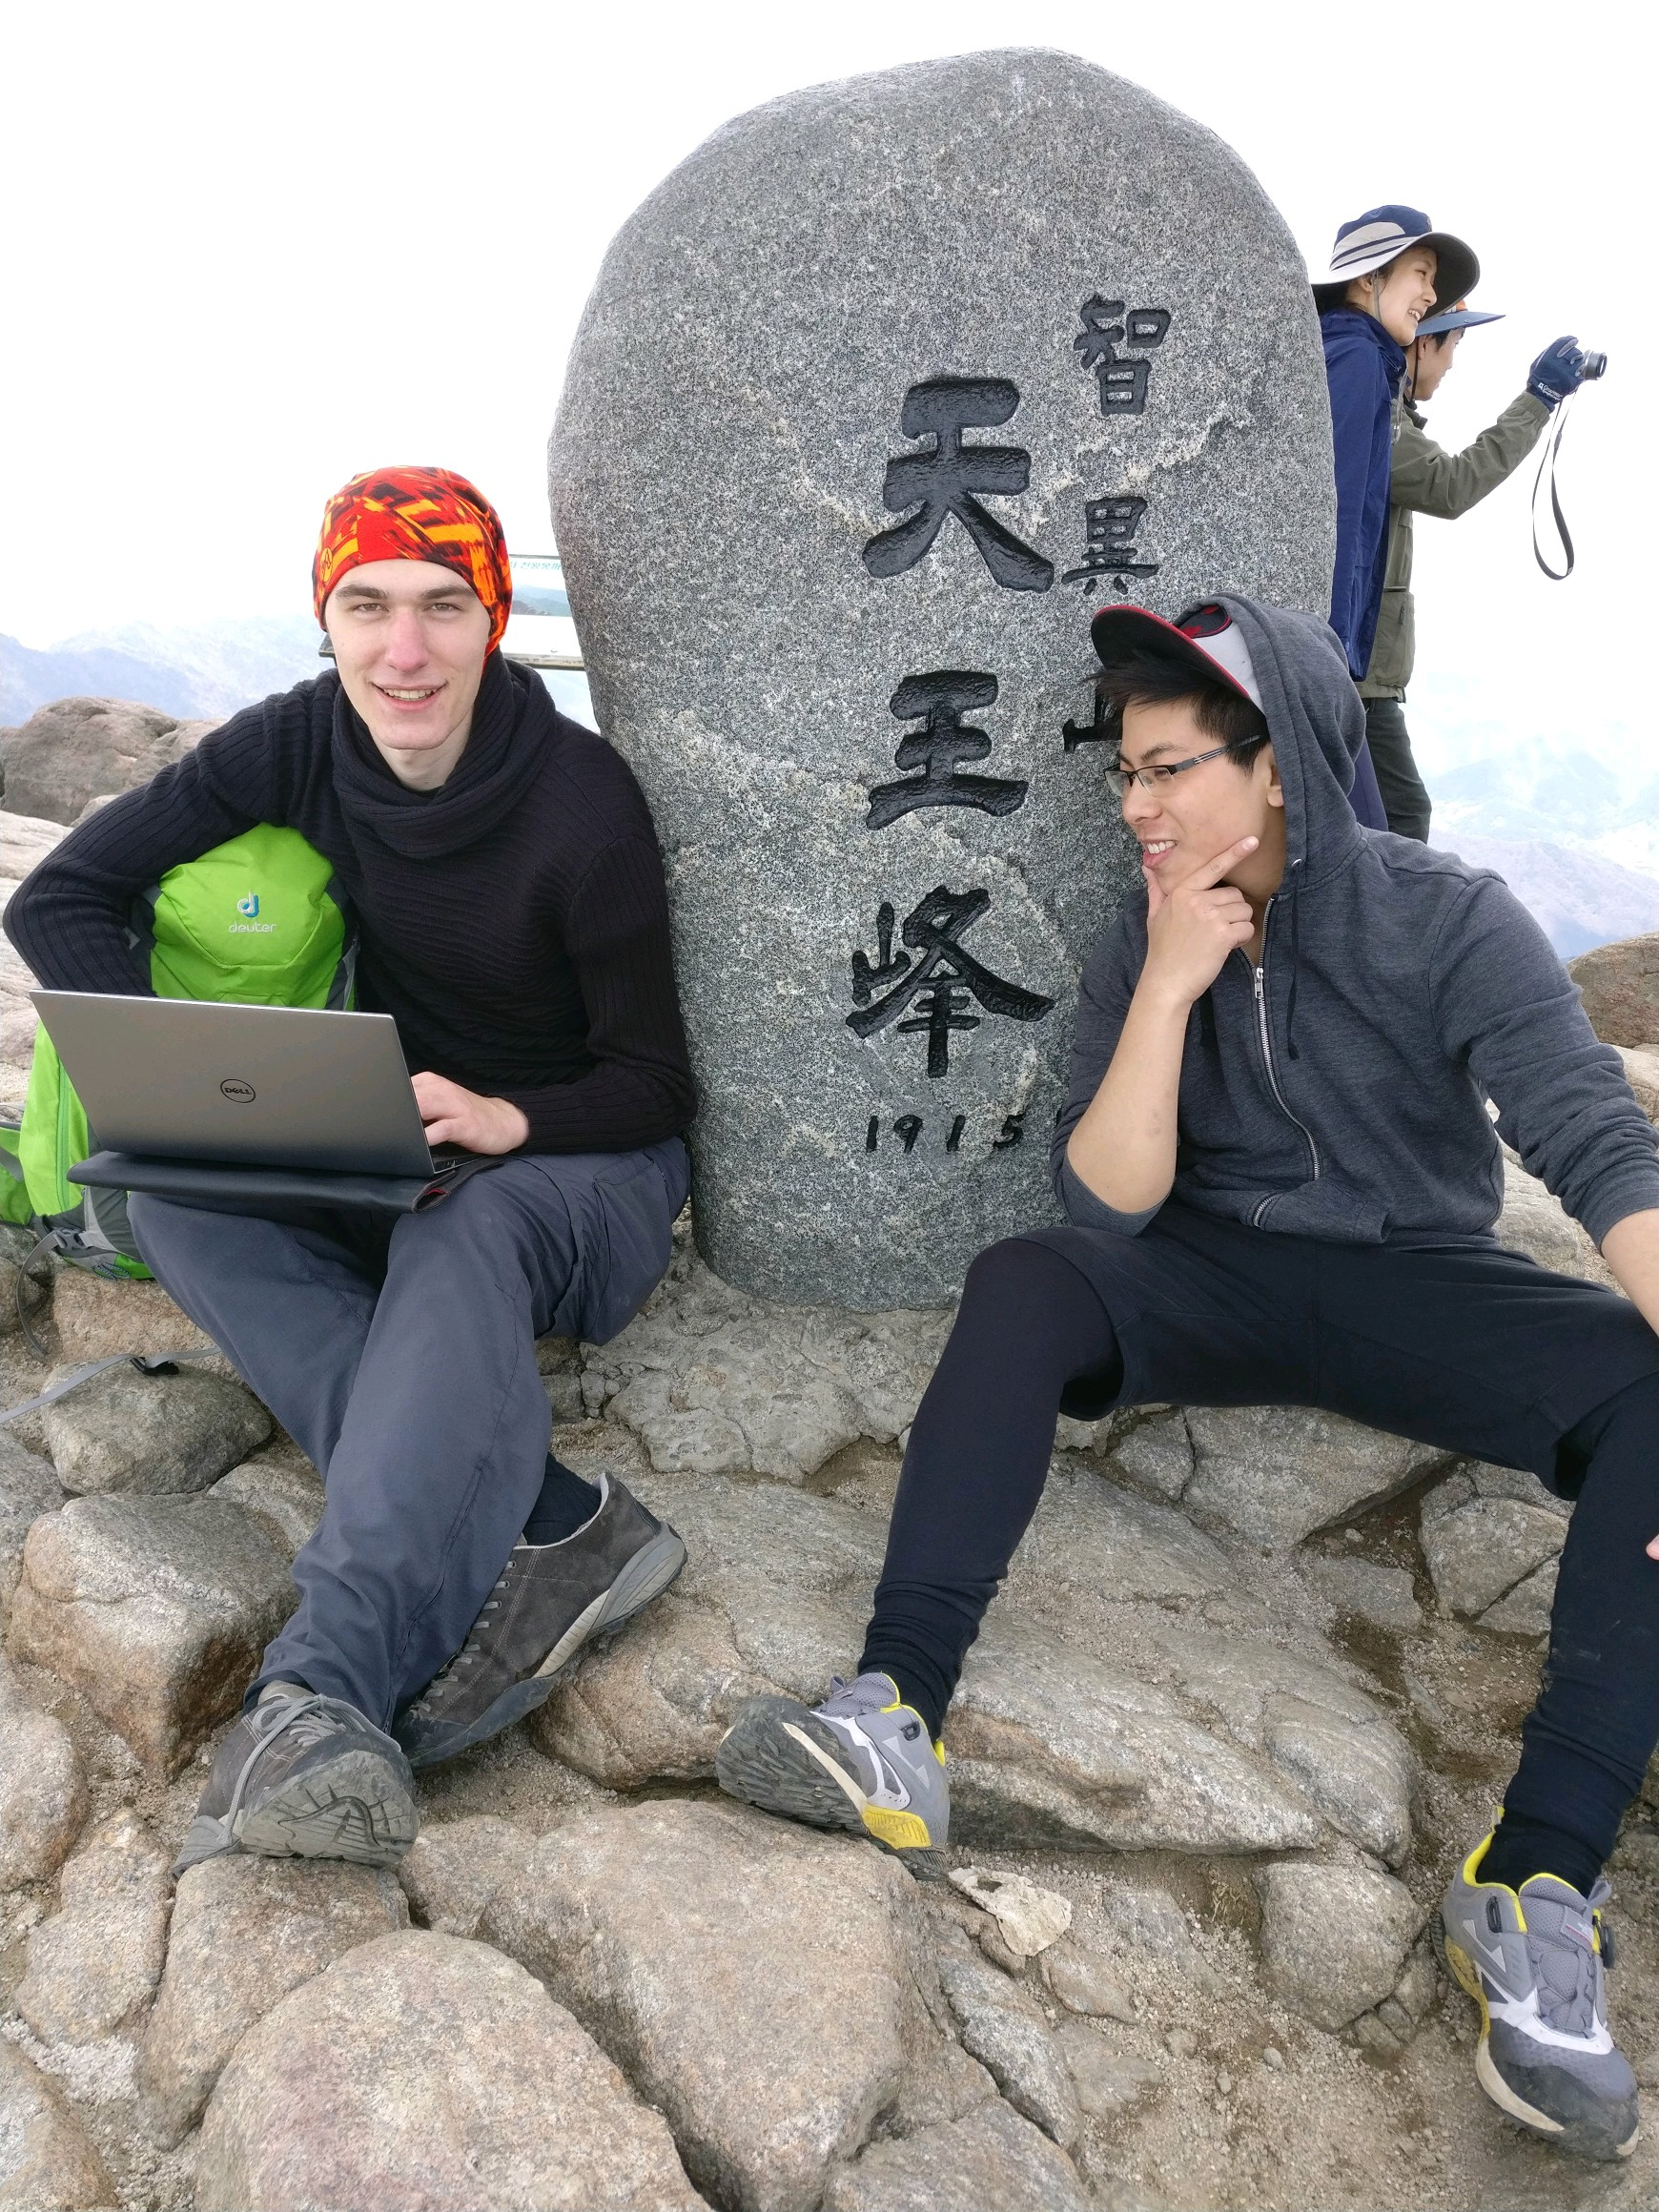
\includegraphics[scale=0.1]{img/jirisan.jpeg}}
\end{figure}  
\end{frame}


\begin{frame}
\frametitle{Architecture of our Implementation}
\begin{figure}[htp] \centering{
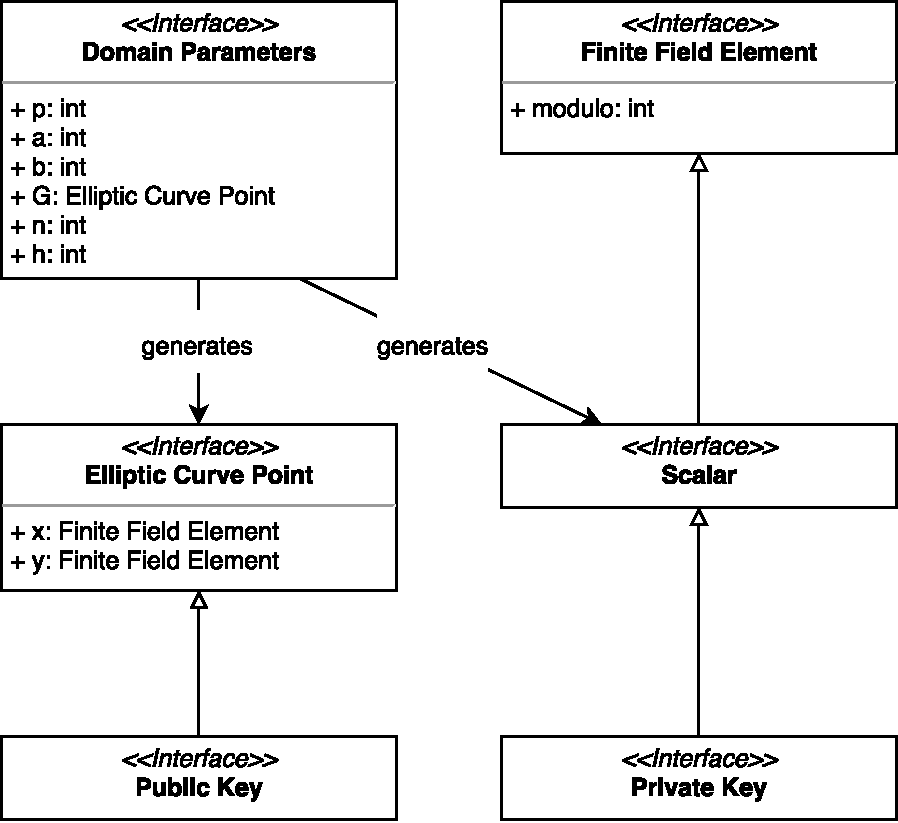
\includegraphics[scale=0.5]{img/architecture.pdf}}
\caption{Class Diagram of our Implementation}
\end{figure}  
\end{frame}

\begin{frame}{Lessons Learned}
\end{frame} 

\begin{frame}[t,allowframebreaks]
	\frametitle{References}
	\printbibliography
\end{frame}

\end{document}